\documentclass[11pt]{article}
\usepackage[utf8]{inputenc}
\usepackage{amsmath,amsthm,amssymb,algorithm,hyperref,xcolor}
\usepackage[noend]{algpseudocode}
\usepackage{subcaption}
\usepackage{graphicx}
\usepackage{wrapfig}
\usepackage[top=0.75in,bottom=0.75in,left=0.75in,right=0.75in,
centering,letterpaper]{geometry}

\title{\vspace{-5ex} Distributed Ensembles for Image Classification}
\usepackage{comment}
\author{Andrea Burns \and Gavin Brown \and Iden Kalemaj}
\date{\vspace{-5ex}}
\newcommand{\cP}{\mathcal{P}}
\newcommand{\cD}{\mathcal{D}}
\newcommand{\cR}{\mathcal{R}}
\newcommand{\cS}{\mathcal{S}}
\newcommand{\cN}{\mathcal{N}}
\newcommand{\N}{\mathbb{N}}
\newcommand{\R}{\mathbb{R}}
\newcommand{\E}{\mathbb{E}}
\newcommand{\eps}{\varepsilon}
\newtheorem{theorem}{Theorem}
\newtheorem{conjecture}[theorem]{Conjecture}
\newtheorem{lemma}[theorem]{Lemma}
\newtheorem{claim}[theorem]{Claim}
\newtheorem{corollary}[theorem]{Corollary}
\newtheorem{definition}[theorem]{Definition}
\newtheorem{proposition}[theorem]{Proposition}
\newtheorem{fact}[theorem]{Fact}
\newtheorem{example}[theorem]{Example}
\newtheorem{assumption}[theorem]{Assumption}
\newtheorem{observation}[theorem]{Observation}
\newtheorem{remark}[theorem]{Remark}

\newcommand{\Sec}[1]{\hyperref[sec:#1]{Section\,\ref*{sec:#1}}} %section
\newcommand{\Obs}[1]{\hyperref[obs:#1]{Observation~\ref*{obs:#1}}} %section
\newcommand{\Eqn}[1]{\hyperref[eq:#1]{Eq. (\ref*{eq:#1})}} %equation
\newcommand{\Fig}[1]{\hyperref[fig:#1]{Fig.\,\ref*{fig:#1}}} %figure
\newcommand{\Tab}[1]{\hyperref[tab:#1]{Table\,\ref*{tab:#1}}} %table
\newcommand{\Thm}[1]{\hyperref[thm:#1]{Theorem\,\ref*{thm:#1}}} %theorem
\newcommand{\Fact}[1]{\hyperref[fact:#1]{Fact\,\ref*{fact:#1}}} %fact
\newcommand{\Lem}[1]{\hyperref[lem:#1]{Lemma\,\ref*{lem:#1}}} %lemma
\newcommand{\Prop}[1]{\hyperref[prop:#1]{Prop.~\ref*{prop:#1}}} %property
\newcommand{\Cor}[1]{\hyperref[cor:#1]{Corollary~\ref*{cor:#1}}} %corollary
\newcommand{\Conj}[1]{\hyperref[conj:#1]{Conjecture~\ref*{conj:#1}}} %conjecture
\newcommand{\Def}[1]{\hyperref[def:#1]{Definition~\ref*{def:#1}}} %
\newcommand{\Alg}[1]{\hyperref[alg:#1]{Algorithm~\ref*{alg:#1}}} %algorithm
\newcommand{\Pro}[1]{\hyperref[pro:#1]{Procedure~\ref*{pro:#1}}} %procedure
\newcommand{\Ex}[1]{\hyperref[ex:#1]{Ex.~\ref*{ex:#1}}} %example
\newcommand{\Clm}[1]{\hyperref[clm:#1]{Claim~\ref*{clm:#1}}} %example
\newcommand{\Stp}[1]{\hyperref[step:#1]{Step~\ref*{step:#1}}}
\newcommand{\Ch}[1]{\hyperref[chap:#1]{Chapter~\ref*{chap:#1}}}


\algnewcommand\algorithmicinput{\textbf{INPUT:}}
\algnewcommand\INPUT{\item[\algorithmicinput]}
\algnewcommand\algorithmicoutput{\textbf{OUTPUT:}}
\algnewcommand\OUTPUT{\item[\algorithmicoutput]}

\begin{document}
\maketitle
\begin{itemize}
	\item \textbf{Github link:} https://github.com/gavinrbrown1/distributed-ensemble-project
	\item \textbf{Slice name:} Project5
\end{itemize}
\vspace{-2ex}
\section{Introduction}

The general goal of image classification is to determine which of several fixed classes an image belongs to. 
One common benchmark is the CIFAR-10 dataset \cite{cifar10}, which contains 32$\times$32 pixel images of ten different classes: airplanes, automobiles, birds, cats, deer, dogs, frogs, horse, ship, truck.
We've included a selection of these images in Figure~\ref{fig:cifar10_images}.
Image classification is an important machine learning task, as it is an initial step toward visual scene understanding. 

Ensembling is a popular way to improve the performance of a machine learning task; an ensemble is a set of different classifiers that are ‘combined’ to make a collective, better decision on the task. 
Such models are also sometimes called ``committees;'' for a reference see Chapter 14 of \cite{bishop}.
%The core idea is that combining many weak learners results in a strong learner. 
In this experiment we distribute 4 independent classifiers across different network nodes (servers) and take a majority vote of their decisions as the final classification result.
This distributed system allows us to investigate latency versus accuracy: by only taking the votes from classifiers that have responded within a certain timeout period, we force decisions to be faster but possibly lose accuracy.
Lastly, we try hand-crafted caching tools that can act as short-cut decisions, to see the impact on end-to-end delay.

\begin{wrapfigure}{r}{0.5\textwidth}
    \centering
    \begin{subfigure}[b]{0.15\textwidth}
        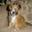
\includegraphics[width=\textwidth]{image0.jpeg}
    \end{subfigure}
    ~
    \begin{subfigure}[b]{0.15\textwidth}
        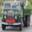
\includegraphics[width=\textwidth]{image3.jpeg}
    \end{subfigure}
    \caption{A few images from CIFAR-10.}
    \label{fig:cifar10_images}
\end{wrapfigure}

\begin{figure}
    \centering
    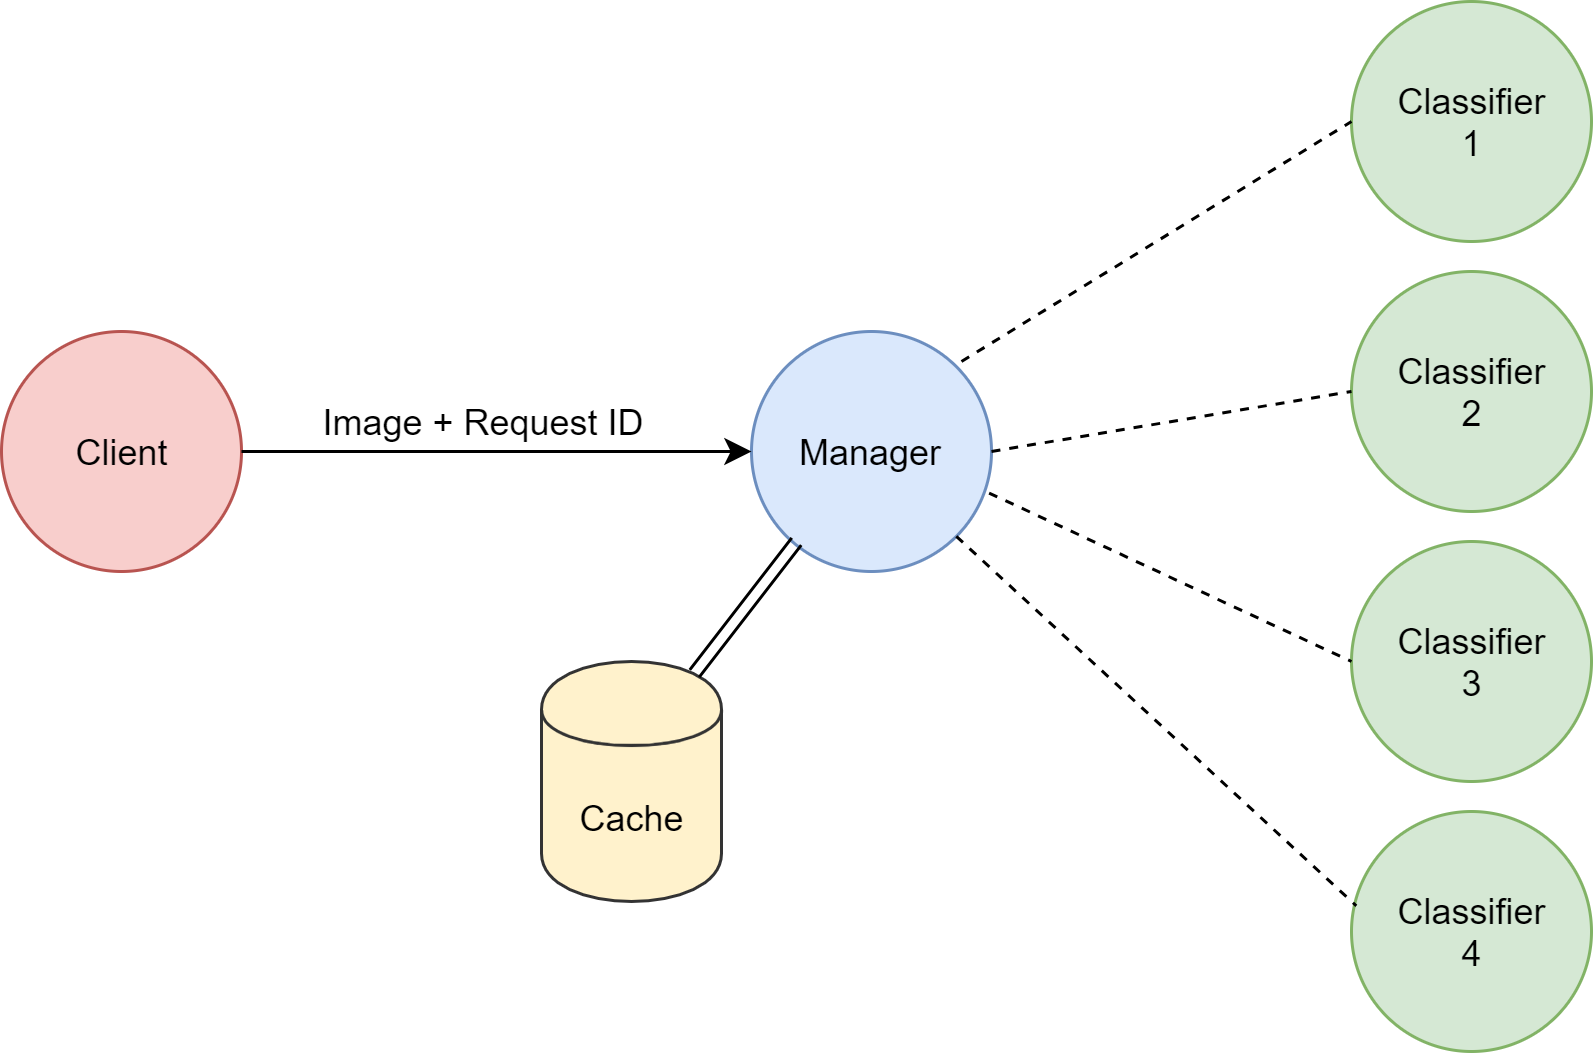
\includegraphics[scale=0.15]{networksArchitecture.png}
    \caption{A high level representation of the GENI architecture setup. The primary components include a client, a manager, a caching mechanism which resides on the manager, and four classifiers which the manager can communicate with.}
    \label{fig:architecture}
\end{figure}

A client wishing to receive classification for an image connects to a manager and sends the image to the manager. The manager then checks if the cache can be utilized before sending copies of the image to the classifiers. If the image already exists in the cache, or a close enough image exists, then it can simply return the cached decision. Otherwise, the manager will start communication with all four classifiers and will aggregate their results into a majority vote. This decision will then be added to the cache and communicated back to the waiting client. The architecture flow can be view in Figure~\ref{fig:architecture}.

The learning outcomes of this project include: greater experience with the featured aspects of computer networking like sockets, caching, and coordinating distributed systems.
We also hope to improve our ability to collaborate on building moderate-scale computer systems from near-scratch, learning more about how to design our solutions.
Finally, we hope to better understand how distributed approaches may benefit machine learning prediction systems.

\section{Experimental methodology}

\subsection{Caching and Sampling}


\begin{figure}[t]
    \centering
    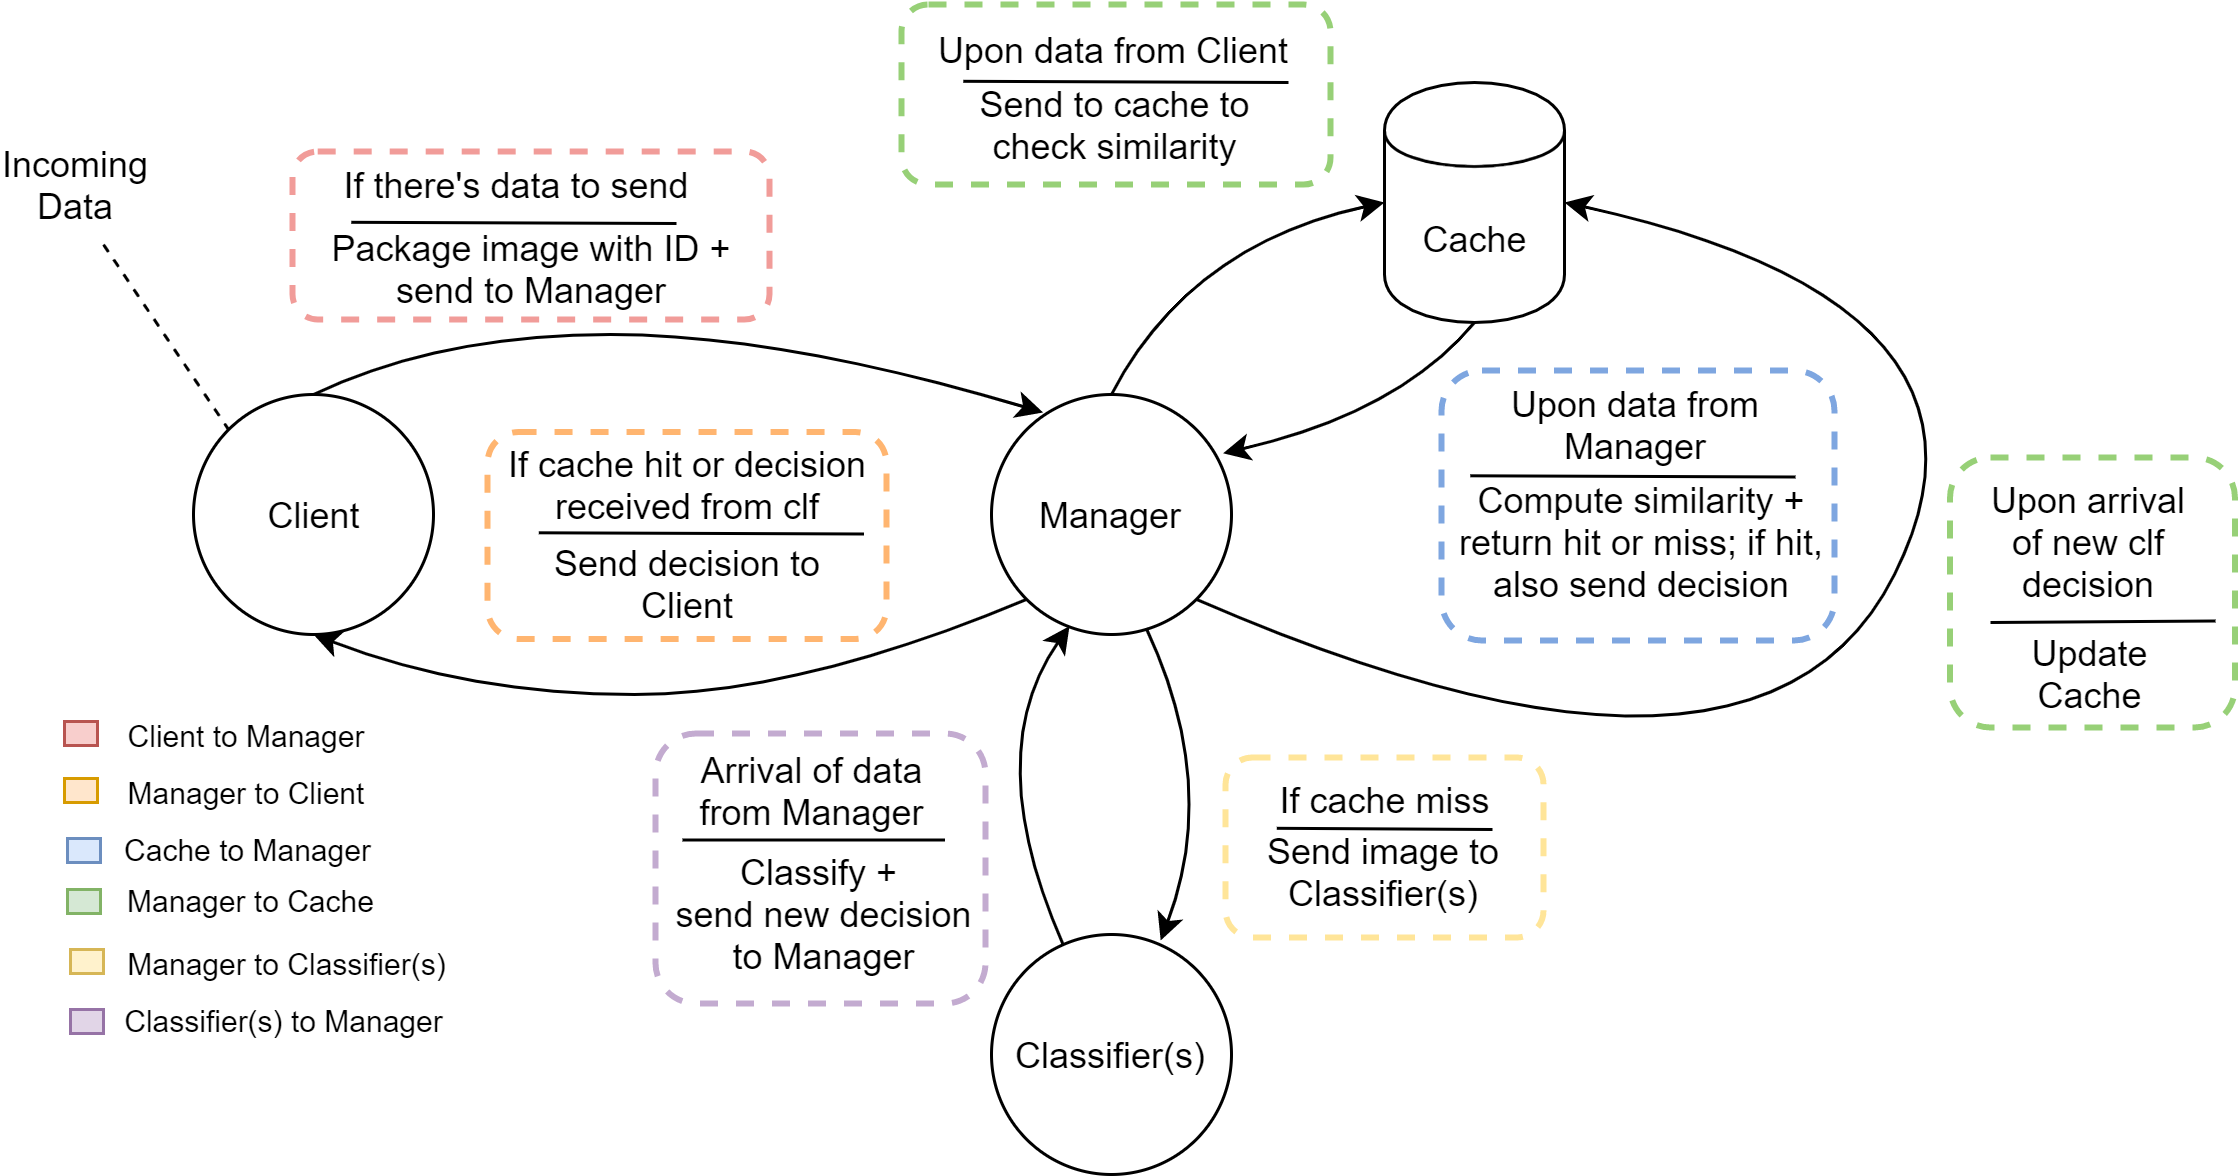
\includegraphics[scale=0.15]{FSM.png}
    \caption{Finite State Machine characterizing the behavior of our system. The classifiers are grouped under the same state since they behave identically up to randomness.}
    \label{fig:fsm}
\end{figure}

The two key components of the cache are how we compare a new image from the client to the existing cache images, and how we choose to update the cache over time. To compare a new image to the cache images, the Zero-Normalized Cross-Correlation coefficient (ZNCC) is used. This is a image similarity metric that is invariant to brightness differences; its values range $[0,1]$, where a ZNCC value of one means the two images being compared are the same. We deem two images similar enough to use the cached decision if their ZNCC is greater than $0.9$. In the case that this threshold is not reached, we do not use the cache and have to communicate with the classifiers. Any time there is a cache miss, the new image is going to be added to the cache once the ensembled decision arrives. We experiment with cache sizes of 15 and 30 to see the effects on latency. 

Once the cache is full, we decide to kick out the \textbf{pair} of closest images in terms of L2/Euclidean distance. We can think of this pair as being the least informative, since they are most similar to each other. Pairwise distances are only updated as samples are added or removed to the cache, never redundantly re-computing pairwise distances.

To evaluate the impact of caching on latency, we consider two models for generating image requests from the client. In the first model images are sampled uniformly at random. In a real system, though, some images may occur far more than others, such as security systems evaluating the same fixed scene. To model this we also sample from a ``long-tailed'' distribution, a simple form of Zipf distribution discussed in \cite{mitzenmacher}, so some image requests will be very frequent over time and the cache will be more useful.

\subsection{Corruption and Delay}

One of the benefits of ensembling, from a networks perspective, is the resilience to delays and corruption experienced in the communication between servers. Specifically, if one or some of the classifiers timeout, the manager can use the decision from those classifiers that did not timeout and still send a response to the client. Similarly, if one or some of the decisions form the classifiers gets corrupted, the use of the majority vote guarantees that the decision of the manager will not loose too much in accuracy. Our experiment considers the following parameters:

\begin{itemize}
	\item a fixed delay experienced by each classifier, set to 0.1s – this simulates the fact that there is a delay in the communication between classifier and manager, and in specific, this delay is longer than the time it takes to check the the cache for an existing decision 
	\item a random delay experienced by three of the classifiers – three classifiers simulates a delay from an exponential distribution with a specified mean, on top of the fixed delay. We consider the following means: 0.1s, 0.2s, 0.3s, 0.4s. This simulates situations with high traffic and slow communication in the network. The fourth classifier does not experience any delay, to guarantee that the manager receives at least one decision before timeout. 
	\item a corruption probability – each classifier experiences corruption, i.e. it sends a flipped decision to the manager, different from the real decision, with some probability. We consider the following corruption probabilities: 0.0, 0.1, 0.2, 0.3. 
	\item 	a timeout – the manger waits for a response form each classifier for 3 seconds only and closes the connection if there is a timeout. 
\end{itemize}
In our experiment we consider the following relationships:

\begin{itemize}
	\item How does accuracy of the classification change with the corruption probability?
	\item How does total communication time, from when the client sends an image, until it receives a classification, change with random delay?
	\item  How does accuracy change with the random delay introduced in the channel between manager and classifier?
\end{itemize}



\section{Results}

\subsection{Usage Instructions}

Our system is designed to be used as part of an automated system, so the process are all started from within scripts. Once the resources are set up on GENI, the user specifies the parameters of the experiments they wish to run in a .csv file residing in the client. The user then starts a script on each machine using the command: python [insert script name] [insert port number]. Once the scripts are running, messages are printed on each node to indicate the communication flow and messages being exchanged, as demonstrated in \ref{fig:client_screenshot}. Refer to the instructions document for a detailed description of how to setup experiments and tweak other parameters. 

\begin{figure}[t]
	\centering
	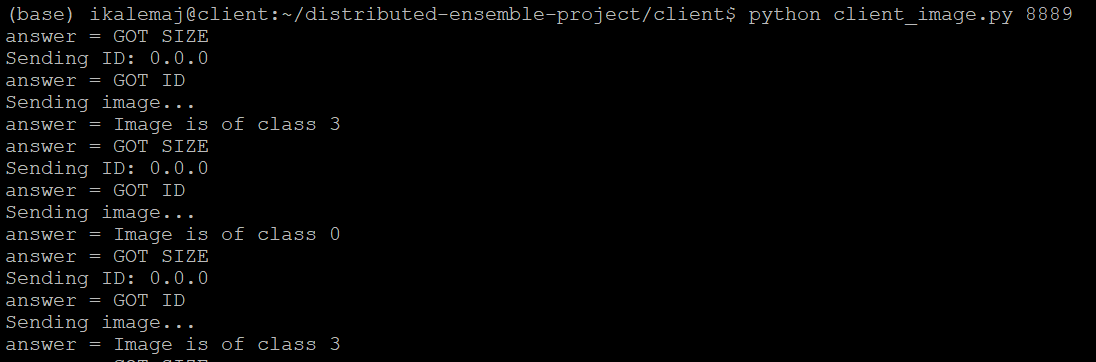
\includegraphics[scale=0.8]{client_screenshot.png}
	\caption{Messages printed on client during experiment}
	\label{fig:client_screenshot}
\end{figure}

\subsection{Analysis Results}

\begin{wraptable}{l}{0.27\textwidth}
    \begin{tabular}{|c|c|c|}
        \hline
        Cache &  Unif. &  Power \\ \hline \hline
        15 & 1.69 & 1.27 \\ \hline
        30 & 2.11 & 1.53 \\ \hline
    \end{tabular}
    \caption{Average communication times, in seconds.}% for different cache sizes and sampling distributions: uniform and the power law $p(i)\propto \frac {1}{i}$.}
    \label{tab:cache}
\end{wraptable}

As you can see in Figure~\ref{fig:results}, our system's behavior changed significantly with different parameters.
On the top left, we can see that decreasing the reliability of our individual classifiers reduced the overall accuracy, but by a lower amount: 
    even when each classifier had a 30\% chance of answering randomly, our average accuracy was over 80\%.
On the top right we see how random delays affect communication time: as expected, they increase it!
On the bottom left we see how random delays affect accuracy (through the timeout mechanism).
This is a little hard to interpret - it's possible more experiments are needed.
On the bottom left we visualize how the cache is used over time: while the uniform distribution rarely gets used, the power law linearity means roughly one in three requests hits the cache.

Table~\ref{tab:cache} that the uniform sampling utilized the cache at a lower rate than the power law.
The smaller cache was faster, possibly because of the overhead of recomputing.

\begin{figure}[h]
    \centering
    \begin{subfigure}{0.45\textwidth}
        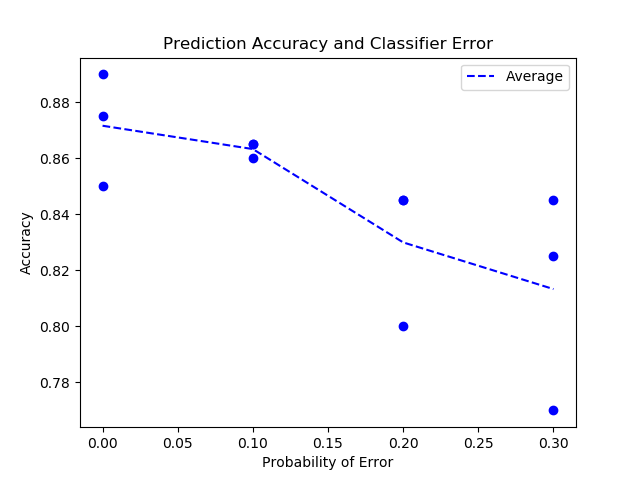
\includegraphics[width=\textwidth]{plot_1_final.png}
    \end{subfigure}
    ~
    \begin{subfigure}{0.45\textwidth}
        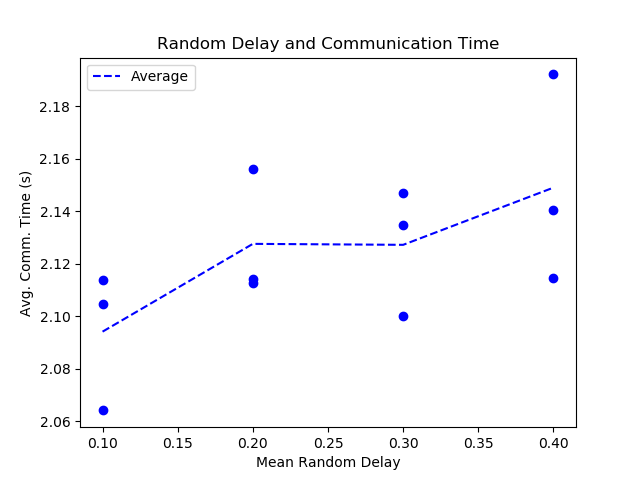
\includegraphics[width=\textwidth]{plot_3_final.png}
    \end{subfigure}
    \\
    \begin{subfigure}{0.45\textwidth}
        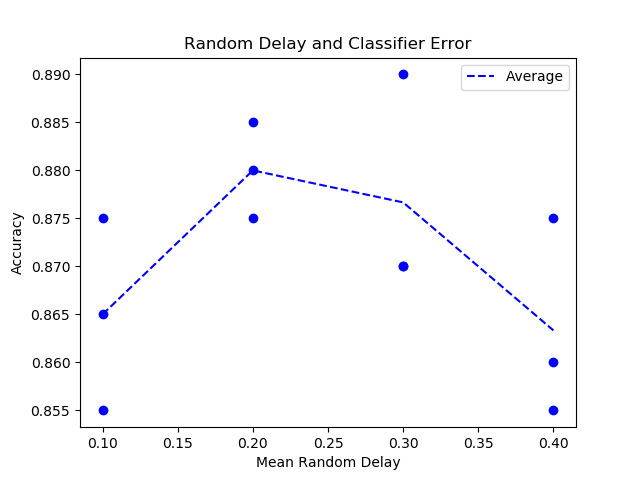
\includegraphics[width=\textwidth]{plot_2_final.png}
    \end{subfigure}
    ~
    \begin{subfigure}{0.45\textwidth}
        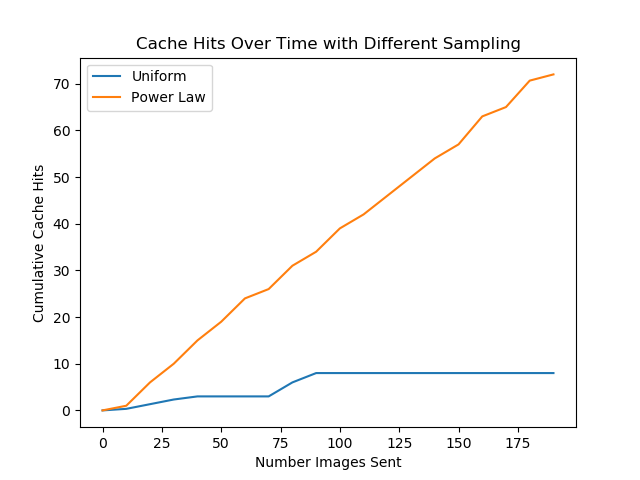
\includegraphics[width=\textwidth]{cache_over_time.png}
    \end{subfigure}
    \caption{Results from various experiments, as described in the text.}
    \label{fig:results}
\end{figure}



\section{Conclusions and Future Extensions}

We found that developing this system and running the experiments was a very rewarding process.
It was enjoyable to see the natural way our research interests of vision, machine learning, and probabilistic algorithms mapped neatly onto the concepts we've learned in class.
We also learned a lot through the process of pulling together the many components and defining our own protocols to interact across machines.
The results mostly matched what we expected, showing clear tradeoffs between accuracy, space requirements, and latency.

{\bf Was anything in the plots surprising?
Probably something should have surprised us.}

Several natural extensions present themselves.
Currently we use a fixed number of classifiers, but we could extend our system to gracefully scale up and down as machines come on and offline.
From the point of the view of the user, we used only one client in order to highlight the effects of the cache and unreliable classification.
We could extend our manager to handle concurrent requests from multiple clients, and set up the classifiers to process images sequentially instead of one over each connection.
Our model also currently sets up a unique TCP connection for each image, but depending on the client's needs it may be more efficient to keep one connection for several images.

\section{Division of labor}

Andrea, Iden, and Gavin decided on the project topic and wrote the proposal and report together.
All high-level decisions were made together: network topology, communication protocols, experiments, etc.
Much of the coding was done in pairs, as well.
The focus of specific sections were as follows: Andrea created the code to control caching.
Iden wrote the bulk of the socket code that allowed the machines to communicate.
Gavin wrote the code to handle the prediction as well as modeling error and delay on the part of the classifier.


\footnotesize\begin{thebibliography}{1}
    \bibitem{bishop}
    Bishop, Christopher M. Pattern recognition and machine learning. Springer, 2006.

    \bibitem{cifar10}
    Krizhevsky, Alex, and Geoffrey Hinton. Learning multiple layers of features from tiny images. Vol. 1. No. 4. Technical report, University of Toronto, 2009.

    \bibitem{mitzenmacher}
    Mitzenmacher, Michael, and Eli Upfal. Probability and computing: randomization and probabilistic techniques in algorithms and data analysis. Cambridge university press, 2017.

\end{thebibliography}



\end{document}
